\documentclass[areasetadvanced]{scrartcl}

\usepackage[utf8]{inputenc}
\usepackage[T2A]{fontenc}
\usepackage[english,russian]{babel}

\usepackage[footskip=1cm,left=25mm, right=15mm, top=20mm, bottom=20mm]{geometry}
\usepackage{setspace}
\usepackage{amsmath, amssymb} 
\usepackage{graphicx}
\usepackage{tikz}
\usetikzlibrary{arrows.meta}
\usepackage{float}
\usepackage{dashrule}
\usepackage{fancyhdr} 
\usepackage{hyperref} 
\usepackage{parskip}
\usepackage{textcomp, enumitem}
\usepackage{indentfirst}
\usepackage{graphicx}
\usepackage{algorithm}
\usepackage{algpseudocode}
\usepackage{array} 
\usepackage{geometry}
\usepackage{afterpage}
\usepackage{minted}
\setcounter{secnumdepth}{3} 
\setcounter{tocdepth}{3}    
\usepackage{listings} 

\tikzstyle{block} = [rectangle, rounded corners, minimum width=3cm, minimum height=1cm, text centered, draw=black, fill=lightgray]

\setkomafont{sectioning}{\normalfont\bfseries} 
\setkomafont{section}{\normalfont\Large\bfseries}
\setkomafont{subsection}{\normalfont\large\bfseries}
\setkomafont{subsubsection}{\normalfont\large\bfseries}
\setkomafont{paragraph}{\normalfont\large\bfseries} 

\lstset{
  language=Haskell,
  basicstyle=\ttfamily\small,
  keywordstyle=\color{blue}\bfseries,
  stringstyle=\color{red},
  commentstyle=\color{green!70!black},
  numbers=left,
  numberstyle=\tiny,
  stepnumber=1,
  numbersep=10pt,
  showstringspaces=false,
  breaklines=true,
  frame=single
}

\setcounter{tocdepth}{2}
\begin{document}
\sloppy
	\thispagestyle{empty}
	\begin{center}
		\large{МИНОБРНАУКИ РОССИИ} \par
		\vspace{0.3cm}
		\normalsize
		{ФЕДЕРАЛЬНОЕ ГОСУДАРСТВЕННОЕ АВТОНОМНОЕ ОБРАЗОВАТЕЛЬНОЕ УЧРЕЖДЕНИЕ ВЫСШЕГО ОБРАЗОВАНИЯ} \par
		\vspace{0.3cm}
		\textbf{\guillemotleft САНКТ-ПЕТЕРБУРГСКИЙ ПОЛИТЕХНИЧЕСКИЙ}
		\textbf{УНИВЕРСИТЕТ ПЕТРА ВЕЛИКОГО\guillemotright} \par
		\vspace{0.3cm}
		{Институт компьютерных наук и кибербезопасности}\par
		{Высшая школа технологий искусственного интеллекта}\par
	\end{center}
	\vfill
	\begin{center}
		{\large Отчёт по дисциплине \guillemotleft Математическая логика\guillemotright}\par
		{\huge   Лабораторная работа №5 
		
		\guillemotleft Реализация LL(1)-анализатора\guillemotright}\par
            {\huge Вариант \textbf{№14}}
         
	\end{center}
	\vfill
	\begin{flushleft}
		Студент: \hspace{1.8cm} \rule[0pt]{2.5cm}{0.5pt}\hfill Салимли Айзек Мухтар Оглы\par
		\vspace{1.5cm}
		Преподаватель: \hspace{0.55cm} \rule[0pt]{2.5cm}{0.5pt}\hfill  Востров Алексей Владимирович
	\end{flushleft}
	\vspace{0.5cm}
	\begin{flushright}
		\guillemotleft \rule[0pt]{0.8cm}{0.5pt}\guillemotright \rule[0pt]{2cm}{0.5pt} 20\rule[0pt]{0.5cm}{0.5pt} г.
	\end{flushright}
	\vfill
	\begin{center}
		Санкт-Петербург, 2025
	\end{center}
	\newpage
	\tableofcontents
	\newpage
\section*{Введение}
	\addcontentsline{toc}{section}{Введение}

    Задана грамматика:
    \begin{enumerate}
        \item $S'\rightarrow S\$$ ,
        \item $S \rightarrow AaS | b$,
        \item $A \rightarrow CAb | B$,
        \item $B \rightarrow cSa | \epsilon$,
        \item $C \rightarrow c | ab$
    \end{enumerate}

    Необходимо:
    \begin{itemize}
        \item Построить множества FIRST и FOLLOW для каждого нетерминала грамматики и таблицу выбора (lookup table).
        \item Реализовать детерминированный левый анализатор (проверка принадлежности цепочки грамматике).
        \item Назначить семантические действия части заданных продукций.
    \end{itemize}
В качестве семантических действий части заданных продукций был выбран вывод функции printStrLn "вывод цепочки", на Haskell.

\newpage
\section{Математическое описание}
Контекстно-свободные грамматики задаются продукциями следующего вида 
\(A \rightarrow \beta\), где \(A\) — нетерминал, \(\beta\) — произвольная цепочка из терминалов и нетерминалов.

Контекстно-свободной грамматикой называется грамматика, у которой левые части всех продукций являются одиночными нетерминалами. 
Контекстно-свободные грамматики являются грамматиками Хомского типа 2.

Заданная грамматика:
\[
\begin{array}{rcl|rcl}
\multicolumn{3}{c|}{\textbf{Исходная грамматика}} &
\multicolumn{3}{c}{\textbf{Итоговая (LL(1)) грамматика}} \\[2pt]
S' &\;\rightarrow\;& S\$                &
S' &\;\rightarrow\;& S\$ \\[4pt]

S  &\;\rightarrow\;& A\,a\,S \mid b     &
S  &\;\rightarrow\;& A\,a\,S \mid b \\[4pt]

A  &\;\rightarrow\;& C\,A\,b \mid B     &
A  &\;\rightarrow\;& C\,A\,b \mid B \\[4pt]

B  &\;\rightarrow\;& c\,S\,a \mid \epsilon &
B  &\;\rightarrow\;& c\,S\,a \mid \epsilon \\[4pt]

C  &\;\rightarrow\;& c \mid ab          &
C  &\;\rightarrow\;& a \mid b
\end{array}
\]

\bigskip

\paragraph{Причина изменения:}
В исходной грамматике альтернативы
\(
A \rightarrow C\,A\,b
\) и
\(
A \rightarrow B
\)
конфликтовали при LL(1)-анализе:
при выводе нетерминала \(C\) в терминал \(c\) обе альтернативы имели
одинаковый префикс \(\langle c,\dots\rangle\).
Из-за этого в таблице разбора возникало пересечение
\(
\text{FIRST}(C\,A\,b)\cap\text{FIRST}(B)\neq\varnothing.
\)

\paragraph{Сделанное преобразование:}
Изменено правило \(C\to c \mid ab\) на \(C\to a \mid b\).
После этого
\[
\text{FIRST}(C)=\{a,b\},\quad
\text{FIRST}(B)=\{\epsilon,c\},
\]
и пересечение с
\(\text{FIRST}(C\,A\,b)=\{a,b\}\) стало пустым.  
Тем самым грамматика удовлетворяет условию LL(1), и
предиктивный парсер строится без конфликтов.

Преобразование не увеличило мощность описываемого языка
(исключены только строки, начинающиеся одиночным терминалом \(c\)),
но позволило использовать детерминированный LL(1)-анализатор
без возврата и ручного разрешения конфликтов.

\newpage
\section{LL(k)-грамматики}

LL($k$)-грамматики~--- это наиболее общий класс грамматик, позволяющих выполнить нисходящий синтаксический анализ, просматривая входную цепочку слева при восстановлении левого канонического вывода данной терминальной цепочки, заглядывая вперёд по входной цепочке на каждом шаге не более, чем на $k$ символов при принятии решения о том, какой из альтернативных правых частей заменить текущий~--- самый левый~--- нетерминал очередной сентенциальной формы.

Промежуточная цепочка в процессе вывода состоит из цепочки терминалов $wu$, самого левого нетерминала $A$ и недоведённой части $x$.

\begin{figure}[H]
    \centering
    \includegraphics[width=0.9\textwidth]{images/wu.png}
    \caption{LL(k)-грамматика}
    \label{llk}
\end{figure}

\newpage
\section{Множества FIRST и FOLLOW}
\[
\begin{array}{l@{\qquad}c@{\quad}l@{\qquad\qquad}c@{\quad}l}
\text{Нетерминал} && \text{\small FIRST} && \text{\small FOLLOW}\\\hline
S' && \{\,a,\;b,\;c\,\}        && \{\,\$\;\} \\[4pt]
S  && \{\,a,\;b,\;c\,\}        && \{\,a,\;\$\;\} \\[4pt]
A  && \{\,a,\;b,\;c,\;\epsilon\,\}     && \{\,a,\;b\,\} \\[4pt]
B  && \{\,c,\;\epsilon\,\}          && \{\,a,\;b\,\} \\[4pt]
C  && \{\,a,\;b\,\}                    && \{\,a,\;b\,\}
\end{array}
\]

\smallskip
\textbf{Замечания.}
\begin{itemize}
  \item Терминал «\$» ― служебный символ конца ввода.
  \item Пустое слово обозначено как \(\epsilon\).
  \item Для \(A\) и \(B\) в {\small FIRST} присутствует \(\epsilon\),
        так как правила \(A\rightarrow B\) и \(B\rightarrow\epsilon\)
        допускают порождение пустой цепочки.
  \item В {\small FOLLOW}(C) попадают \(\{a,b\}\),
        так как после \(C\) в правиле \(A\rightarrow C A b\) стоит
        нетерминал \(A\) (дать его {\small FIRST}\(\setminus\epsilon\)) 
        и терминал \(b\); а из-за наличия \(\epsilon\in\text{\small FIRST}(A)\)
        добавляется и всё {\small FOLLOW}(A).
\end{itemize}

Наша обновлённая грамматика — LL(1), потому что для каждого нетерминала достаточно одного символа look-ahead, чтобы однозначно выбрать альтернативу.
Для любого нетерминала его альтернативы имеют непересекающиеся множества FIRST.
Если у некоторой альтернативы в FIRST находится $\epsilon$
$\epsilon$, то она также непересекается с FOLLOW того же нетерминала.
Тем самым предиктивное множество (FIRST $\cup$ FOLLOW, когда применимо) каждой альтернативы уникально — конфликтов нет.

Эквивалентно этому, при построении «таблицы выбора» (lookup-table) каждая ячейка (нетерминал,символ look-ahead) заполняется не более чем одним правилом; таблица не содержит пересечений — что и подтверждает свойство LL(1).

\[
\begin{array}{|c|c|l|}
\hline
\text{Нетерм.} & \text{look-ahead} & \text{применяемое правило} \\ \hline
S  & a & S \,\rightarrow\, A\,a\,S \\ \hline
S  & b & S \,\rightarrow\, b       \\ \hline
S  & c & S \,\rightarrow\, A\,a\,S \\ \hline
A  & a & A \,\rightarrow\, C\,A\,b \\ \hline
A  & b & A \,\rightarrow\, C\,A\,b \\ \hline
A  & c & A \,\rightarrow\, B       \\ \hline
A  & \text{(}\epsilon\text{)}\!/b & A \,\rightarrow\, B       \\ \hline
B  & c & B \,\rightarrow\, c\,S\,a \\ \hline
B  & a,b, \$  & B \,\rightarrow\, \epsilon \\ \hline
C  & a & C \,\rightarrow\, a      \\ \hline
C  & b & C \,\rightarrow\, b      \\ \hline
\end{array}
\]

\newpage
\section{Левый анализатор LL(1)}
Так как заданная грамматика является LL(1), то для её анализа будет использован LL(1)-анализатор.
LL(1) анализаторы, которые просматривают поток только на один символ вперед при принятии решения о том, какое правило грамматики необходимо применить.

\begin{figure}[H]
    \centering
    \includegraphics[width=0.7\textwidth]{images/llk.png}
    \caption{LL(1)-анализатор}
    \label{ll1}
\end{figure}
Реализован классический анализатор-предиктор с магазинной памятью.
Его стек служит «планом» ещё не выполненной части вывода; элементами стека являются все терминальные и нетерминальные символы грамматики, а также служебный символ \$, обозначающий конец ввода.

\begin{enumerate}
  \item \textbf{Инициализация}\\
  В стек заносится пара $S'\ \$$ (снизу — $\$$, сверху — начальный нетерминал $S'$). Указатель входа ставится на первый терминал обрабатываемой цепочки.

  \item \textbf{Основной цикл}\\
  Пока стек не пуст, рассматриваем символ на его вершине и текущий входной терминал.

  \begin{tabular}{|p{0.38\textwidth}|p{0.55\textwidth}|}
    \hline
    \textbf{Ситуация на вершине стека} & \textbf{Действие анализатора} \\
    \hline
    Терминал совпадает с текущим символом входа & \textit{match}: снимаем терминал со стека, считываем следующий входной символ \\
    Терминал не совпадает & \textit{ошибка}: входная цепочка не соответствует грамматике \\
    Нетерминал $A$ & по паре $(A, a_1)$ смотрим look-up таблицу и находим единственную подходящую продукцию $A \rightarrow \beta$; заменяем $A$ на $\beta$ (символы $\beta$ кладутся в стек в обратном порядке, чтобы первый символ $\beta$ оказался сверху) \\
    Для пары $(A, a_1)$ нет правила & \textit{ошибка} (недопустимый вход) \\
    \hline
  \end{tabular}

  При замене нетерминала сразу выполняется присвоенное ему \textbf{семантическое действие}: из сгенерированных потомками фраз собирается фрагмент Haskell-кода (\texttt{putStrLn "ab"}, \texttt{"c" ++ $\dots$}, и т. д.).

  \item \textbf{Завершение}\\
  Анализ оканчивается успехом, если одновременно выполнены условия:
  \begin{itemize}
    \item стек пуст (всё «расписание вывода» отработано);
    \item входная цепочка исчерпана и последний считанный символ — $\$$.
  \end{itemize}
  В этом случае накопленный семантический атрибут корня ($S'$) возвращается как результирующий Haskell-код.

  \item \textbf{Обнаружение ошибок}\\
  Ошибка фиксируется в двух случаях:
  \begin{itemize}
    \item терминал на вершине стека не совпал с текущим входным символом;
    \item пара (A, a) на вершине не соответствует ни одна запись таблицы выбора для данного look-ahead.
  \end{itemize}
  В программе выводится диагностическое сообщение вида:
  \begin{quote}
    Expected 'a', saw 'c' или No rule for A on 'b'.
  \end{quote}
\end{enumerate}

\newpage
\section{Семантические действия}
\begin{enumerate}
    \item $S  \;\rightarrow\; A\,a\,S$           
    \item $S  \;\rightarrow\; b$             
    \item $A  \;\rightarrow\; C\,A\,b$          
    \item $A  \;\rightarrow\; B$              
    \item $B  \;\rightarrow\; c\,S\,a$         
    \item $B \;\rightarrow\;  \epsilon $          
    \item $C  \;\rightarrow\; a$                 
    \item $C  \;\rightarrow\; b$                
  \end{enumerate}
  
  \vspace{1em}
  \medskip
  \noindent
  Семантические действия формируют фрагменты Haskell-кода, которые:
  \begin{itemize}
    \item Генерируют точки на сетке 400x400 пикселей с разными цветами:
      \begin{itemize}
        \item Синие точки для терминала 'b' (вероятность 0.3)
        \item Зеленые точки для терминала 'c' (вероятность 0.7)
        \item Оранжевые точки для терминалов 'a' и 'b' в правиле C (вероятность 0.5)
      \end{itemize}
    \item Создают случайные стены (40 штук) на сетке, избегая пересечения с точками
    \item Находят кратчайший путь между соседними точками с использованием:
      \begin{itemize}
        \item Окрестности Мура (8 соседних клеток)
        \item Алгоритма поиска в ширину (BFS)
        \item Визуализации пути с анимацией
      \end{itemize}
  \end{itemize}
  
  \bigskip
  \noindent
  \noindent\textbf{Пример цепочки языка:}\; \texttt{bbcbabbab \$}

  \[
  \begin{array}{lcl}
  S' &\Rightarrow& S\ \$                                                   \\[2pt]
     &\Rightarrow& A\,a\,S\ \$                                             \\[2pt]
     &\Rightarrow& C\,A\,b\,a\,S\ \$ \qquad(\text{правило }A\to C\,A\,b)  \\[2pt]
     &\Rightarrow& \underbrace{b}_{C\to b}\,A\,b\,a\,S\ \$                \\[2pt]
     &\Rightarrow& b\,b\,a\,S\ \$ \qquad\qquad\;(\text{правило }A\to\epsilon)\\[2pt]
     &\Rightarrow& b\,b\,a\,\underbrace{b}_{S\to b}\ \$                  \\[2pt]
  \end{array}
  \]
  
  \medskip
  При таком выводе анализатор выполняет семантические действия:
  \begin{itemize}
    \item Генерирует оранжевую точку (правило $C\to b$)
    \item Генерирует синюю точку (правило $S\to b$)
    \item Создает случайные стены на сетке
    \item Находит кратчайший путь между точками
    \item Визуализирует результат на экране
  \end{itemize}

\begin{figure}[H]
    \centering
    \includegraphics[width=0.3\textwidth]{images/tree.png}
    \caption{Дерево для цепочки bbcbabbab \$}
    \label{tree}
\end{figure}

Если рассматривать стек, и цепочку - bbcbabbab:

\newcommand{\stk}[1]{\texttt{#1}}  

\[
\begin{array}{|c|l|l|}
\hline
\textbf{Шаг} &
\multicolumn{1}{c|}{\textbf{Стек (сверху $\to$ вниз)}} &
\multicolumn{1}{c|}{\textbf{Оставшийся ввод}} \\ \hline
0 & \stk{S'\ \$}                       & \stk{bbcbabbab \$} \\ \hline
1 & \stk{S\ \$}                        & \stk{bbcbabbab \$} \\ \hline
2 & \stk{A\ a\ S\ \$}                  & \stk{bbcbabbab \$} \\ \hline
3 & \stk{C\ A\ b\ a\ S\ \$}            & \stk{bbcbabbab \$} \\ \hline
4 & \stk{b\ A\ b\ a\ S\ \$}            & \stk{\color{red}{b}\ bcbabbab \$} \\ \hline
5 & \stk{b\ b\ a\ S\ \$}               & \stk{\color{red}{b}\ bcbabbab \$} \\ \hline
6 & \stk{b\ b\ a\ b\ \$}               & \stk{\color{red}{b}\ bcbabbab \$} \\ \hline
7 & \stk{b\ b\ a\ \$}                  & \stk{\color{red}{c}\ babbab \$} \\ \hline
8 & \stk{b\ b\ a\ B\ \$}               & \stk{\color{red}{c}\ babbab \$} \\ \hline
9 & \stk{b\ b\ a\ c\ S\ a\ \$}         & \stk{\color{red}{c}\ babbab \$} \\ \hline
10 & \stk{b\ b\ a\ c\ b\ a\ \$}        & \stk{\color{red}{b}\ abbab \$} \\ \hline
11 & \stk{b\ b\ a\ c\ b\ \$}           & \stk{\color{red}{a}\ bbab \$} \\ \hline
12 & \stk{b\ b\ a\ c\ \$}              & \stk{\color{red}{b}\ bab \$} \\ \hline
13 & \stk{b\ b\ a\ \$}                 & \stk{\color{red}{b}\ ab \$} \\ \hline
14 & \stk{b\ b\ \$}                    & \stk{\color{red}{a}\ b \$} \\ \hline
15 & \stk{b\ \$}                       & \stk{\color{red}{b}\ \$} \\ \hline
16 & \stk{\$}                          & \stk{\color{red}{\$}} \\ \hline
17 & \textit{стек пуст}                & \textit{достиг конца} \\ \hline
\end{array}
\]

\bigskip
\noindent
В столбце \textbf{Стек} верхняя строка — вершина.\;
Красным выделен текущий символ входа, который
либо сравнивается с вершиной, либо определяет выбор продукции.

Разбор завершается на шаге 17: стек опустел, входная
строка полностью обработана — цепочка \texttt{bbcbabbab \$} принята.
\newpage
\section{Программная реализация}
Для реализации LL(1)-анализатора был создан cabal проект со следующей структурой:
\begin{itemize}
  \item \texttt{Lib.hs}: модуль с реализацией LL(1)-анализатора и генерации точек;
  \item \texttt{Main.hs}: GUI-интерфейс программы;
  \item \texttt{Язык программирования}: Haskell
  \item \texttt{Конфигурация языка}: Haskell2010
  \item \texttt{Среда разработки}: Cursor IDE
\end{itemize}

Файл Lib.hs:
\begin{lstlisting}
  {-# LANGUAGE LambdaCase #-}
  {-# LANGUAGE ParallelListComp #-}
  {-# OPTIONS_GHC -Wall #-}
  
  module Lib
    ( NonTerm(..)
    , Production(..)
    , grammar
    , firstSets, followSets, parseTable
    , printFirstSets, printFollowSets, printParseTable
    , parse                     
    , genStrings
    , saveGeneratedStringsToFile
    , loadGeneratedStrings
    , genInteract
    , setup                     
    , pause
    ) where
  
  import           Data.List       (intercalate, tails, isPrefixOf, minimumBy)
  import           Data.Map.Strict (Map)
  import qualified Data.Map.Strict as M
  import           Data.Set        (Set)
  import qualified Data.Set        as S
  import           System.IO       (writeFile, readFile, hFlush, stdout)
  import           System.IO.Unsafe (unsafePerformIO)
  import           System.Directory (doesFileExist)
  import qualified Graphics.UI.Threepenny as UI
  import           Graphics.UI.Threepenny.Core
  import qualified Graphics.UI.Threepenny.Canvas as UI
  import           Graphics.UI.Threepenny.Canvas (Point(..))
  import           Control.Monad   (replicateM, forM_, forM, void)
  import           System.Random   (randomRIO)
  import           Data.IORef      (newIORef, readIORef, writeIORef)
  import           Data.Ord        (comparing)
  import           Data.Maybe      (fromMaybe)
  import           Control.Concurrent (threadDelay)
  
  
  prompt :: String -> IO ()
  prompt s = putStr s >> hFlush stdout
  
  pause :: IO ()
  pause = putStrLn "Press Enter to continue..." >> void getLine
  
  
  data NonTerm = S' | S | A | B | C deriving (Eq, Ord, Show)
  data Symbol  = NT NonTerm | T String | Eps deriving (Eq, Ord, Show)
  
  data Production = P { lhs :: NonTerm, rhs :: [Symbol], act :: [String] -> String }
  
  
  codeB, codeC, codeAB :: String
  codeB  = "  generatePixel 0.3 >>= \\p -> print p\n"
  codeC  = "  generatePixel 0.7 >>= \\p -> print p\n"
  codeAB = "  generatePixel 0.5 >>= \\p -> print p\n"
  
  grammar :: [Production]
  grammar =
    [ P S' [NT S, T "$"]               (\[s,_]   -> "main :: IO ()\nmain = do\n" <> s)
    , P S  [NT A, T "a", NT S]         (\[a,_,s] -> a <> s)
    , P S  [T "b"]                     (const codeB)
    , P A  [NT C, NT A, T "b"]         (\[c,a,_] -> c <> a)
    , P A  [NT B]                      (\[b]     -> b)
    , P B  [T "c", NT S, T "a"]        (\[_,s,_] -> codeC <> s)
    , P B  [Eps]                       (const "")
    , P C  [T "a"]                     (const codeAB)
    , P C  [T "b"]                     (const codeAB)
    ]
  
  nonterms :: [NonTerm]
  nonterms = [S',S,A,B,C]
  
  type FirstSets = Map NonTerm (Set String)
  type FollowSets = Map NonTerm (Set String)
  type Key = (NonTerm,String)
  type ParseTable = Map Key Production
  
  aempty :: Set String; aempty = S.empty
  
  firstSets :: FirstSets
  firstSets = fixedPoint step (M.fromList [(n,aempty) | n<-nonterms])
    where
      step tbl = foldl upd tbl grammar
        where upd acc (P nt B _) = M.insertWith S.union nt (firstSeq B tbl) acc
  
  firstSeq :: [Symbol] -> FirstSets -> Set String
  firstSeq []          _   = S.singleton ""
  firstSeq (Eps:_)     _   = S.singleton ""
  firstSeq (T t:_)     _   = S.singleton t
  firstSeq (NT n:B) tbl =
    let f = M.findWithDefault aempty n tbl
    in if S.member "" f then S.delete "" f `S.union` firstSeq B tbl else f
  
  followSets :: FollowSets
  followSets = fixedPoint step start
    where
      start = M.insert S' (S.singleton "$") (M.fromList [(n,aempty) | n<-nonterms])
      step tbl = foldl proc tbl grammar
        where
          proc acc (P nt B _) = foldl (prop nt) acc (zip B (map tail $ tails B))
          prop pnt acc (NT a, suf) =
            let fB = firstSeq suf firstSets
                acc1 = M.insertWith S.union a (S.delete "" fB) acc
            in if S.member "" fB || null suf
                 then M.insertWith S.union a (M.findWithDefault aempty pnt tbl) acc1
                 else acc1
          prop _ acc _ = acc
  
  parseTable :: ParseTable
  parseTable = foldl add M.empty grammar
    where
      add acc p@(P nt B _) = foldl ins acc sels
        where
          fB = firstSeq B firstSets
          sels = if S.member "" fB
                   then S.delete "" fB `S.union` M.findWithDefault aempty nt followSets
                   else fB
          ins m tok = case M.lookup (nt,tok) m of
                        Nothing -> M.insert (nt,tok) p m
                        Just _  -> error $ "LL(1) conflict at " ++ show (nt,tok)
  
  type Result = (String,[String])
  
  splitTokens :: String -> Either String [String]
  splitTokens s = 
    let invalid = filter (`notElem` "abc") s
    in if null invalid 
       then Right $ map (:[]) s
       else Left $ "Invalid characters found: " ++ show invalid
  
  
  parseS :: [String] -> [Result]
  parseS toks = s_b toks ++ s_AaS toks
    where

      s_b ("b":xs) = [(codeB,xs)]
      s_b _        = []

      s_AaS ts =
        [ (aRes <> sRes, rest2)
        | (aRes, rest1) <- parseA ts
        , ("a":afterA)  <- [rest1]
        , (sRes, rest2) <- parseS afterA
        ]
  
  
  parseA :: [String] -> [Result]
  parseA ts = a_CAb ts ++ a_B ts
    where
      a_CAb xs =
        [ (cRes <> aRes, rest3)
        | (cRes, rest1) <- parseC xs
        , (aRes, rest2) <- parseA rest1
        , ("b":rest3)   <- [rest2] ]
      a_B = parseB
  
  
  parseB :: [String] -> [Result]
  parseB ("c":xs) =
    [ (codeC <> sRes, rest2)
    | (sRes, rest1) <- parseS xs
    , ("a":rest2)   <- [rest1] ]
  parseB ts = [("",ts)]     
  
  
  parseC :: [String] -> [Result]
  parseC ("a":xs) = [(codeAB,xs)]
  parseC ("b":xs) = [(codeAB,xs)]
  parseC _        = []
  
  
  parseTokens :: [String] -> Maybe String
  parseTokens ts =
    case [c | (c,[]) <- parseS ts] of
      (r:_) -> Just r
      _     -> Nothing
  
  parse :: String -> Either String String
  parse inp = do
    tokens <- splitTokens inp
    case parseTokens tokens of
      Just c  -> Right c
      Nothing -> Left "String does not belong to grammar."
  
  
  printFirstSets :: IO ()
  printFirstSets = mapM_ pr (M.toList firstSets)
    where pr (n,s) = putStrLn $ show n ++ " : " ++ show (S.map f s)
          f "" = "eps"; f x = x
  
  printFollowSets :: IO ()
  printFollowSets = mapM_ (\(n,s)->putStrLn $ show n ++ " : " ++ show s)
                          (M.toList followSets)
  
  printParseTable :: IO ()
  printParseTable = mapM_ pr (M.toList parseTable)
    where pr ((nt,tok),P _ B _) =
            putStrLn $ show nt ++ ", '" ++ tok ++ "' => " ++ show B
  
  
  genStrings :: Int -> [[String]]
  genStrings depth = S.toList $ explore depth [[NT S]]
    where
      isNT (NT _) = True; isNT _ = False
      isT  (T _)  = True; isT  _ = False
      toTok (T x) = [x];  toTok _ = []
  
      explore 0 ss = S.fromList [concatMap toTok s | s<-ss, all isT s]
      explore k ss = explore (k-1) (ss >>= expand)
  
      expand s = case break isNT s of
                   (_,[])            -> [s]
                   (pre, NT nt:suf)  -> [pre ++ B ++ suf | B<-alts nt]
  
      alts S' = [[NT S, T "$"]]
      alts S  = [[NT A, T "a", NT S],[T "b"]]
      alts A  = [[NT C, NT A, T "b"],[NT B]]
      alts B  = [[T "c", NT S, T "a"],[]]
      alts C  = [[T "a"],[T "b"]]
  
  fixedPoint :: Eq a => (a->a)->a->a
  fixedPoint f x = let x' = f x in if x'==x then x else fixedPoint f x'
  
  saveGeneratedStringsToFile :: Int -> IO ()
  saveGeneratedStringsToFile d = writeFile "generated_strings.txt"
                               . unlines . map concat $ genStrings d
  
  loadGeneratedStrings :: IO [[String]]
  loadGeneratedStrings = do
    e <- doesFileExist "generated_strings.txt"
    if e then map (map (:[])) . lines <$> readFile "generated_strings.txt"
         else pure []
  
  genInteract :: IO ()
  genInteract = do
    prompt "Depth? "
    dStr <- getLine
    case reads dStr of
      [(d,"")] | d>0 -> mapM_ (putStrLn . concat) (genStrings d)
                         >> saveGeneratedStringsToFile d
      _              -> putStrLn "Not a positive integer."
  
  
  data Pixel = Pixel { x :: Int, y :: Int, color :: String } deriving (Show)
  
  generatePixel :: Double -> IO Pixel
  generatePixel prob = do
    x <- randomRIO (0, 400)
    y <- randomRIO (0, 400)
    let r = floor $ prob * 255
        g = floor $ (1 - prob) * 255
        b = floor $ (prob + 0.5) * 127
    pure $ Pixel x y $ "rgb(" ++ show r ++ "," ++ show g ++ "," ++ show b ++ ")"
  
  
  clearCanvas :: UI.Canvas -> UI ()
  clearCanvas = UI.clearCanvas
  
  data PixelPoint = PixelPoint { px :: Int, py :: Int, pointColor :: String }
                  deriving (Eq, Show)
  type Node = (Int,Int)
  
  drawPoint :: UI.Canvas -> PixelPoint -> UI ()
  drawPoint ctx (PixelPoint x y col) = do
    let gx = (x `div` 10) * 10
        gy = (y `div` 10) * 10
    ctx # set' UI.fillStyle (UI.htmlColor col :: UI.FillStyle)
    _   <- UI.fillRect (fromIntegral gx, fromIntegral gy) 10 10 ctx
    pure ()
  
  drawPath :: UI.Canvas -> [Node] -> UI ()
  drawPath _   []   = pure ()
  drawPath ctx path = do
    ctx # set' UI.fillStyle (UI.htmlColor "rgba(0,0,255,0.3)" :: UI.FillStyle)
    mapM_ (\(x,y)-> UI.fillRect (fromIntegral x,fromIntegral y) 10 10 ctx
                     >> liftIO (threadDelay 100000)) path
  
  drawGrid :: UI.Canvas -> UI ()
  drawGrid ctx = do
    ctx # set' UI.strokeStyle "lightgray"
    ctx # set' UI.lineWidth 1
    forM_ [0,10..400] $ \x -> UI.beginPath ctx >> UI.moveTo (fromIntegral x,0) ctx
                                           >> UI.lineTo (fromIntegral x,400) ctx
                                           >> UI.stroke ctx
    forM_ [0,10..400] $ \y -> UI.beginPath ctx >> UI.moveTo (0,fromIntegral y) ctx
                                           >> UI.lineTo (400,fromIntegral y) ctx
                                           >> UI.stroke ctx
  
  data Wall = Wall { wx :: Int, wy :: Int } deriving (Eq, Ord, Show)
  
  randWall :: Set Node -> IO Wall
  randWall busy = pick
    where
      pick = do
        gx <- randomRIO (0,39)
        gy <- randomRIO (0,39)
        let n = (gx*10,gy*10)
        if S.member n busy then pick else pure (Wall (fst n) (snd n))
  
  generateWalls :: Int -> [Node] -> IO [Wall]
  generateWalls n occ = go n (S.fromList occ) []
    where
      go 0 _ acc = pure acc
      go k busy acc = do
        w@(Wall x y) <- randWall busy
        go (k-1) (S.insert (x,y) busy) (w:acc)
  
  moore :: Node -> [Node]
  moore (x,y) = [(x+dx,y+dy)
                | dx<-[-10,0,10], dy<-[-10,0,10], (dx,dy)/=(0,0)]
  
  inField :: Node -> Bool
  inField (x,y) = x>=0 && x<=390 && y>=0 && y<=390
  
  bfs :: Set Node -> Node -> Node -> Maybe [Node]
  bfs walls start goal = go S.empty (S.singleton start) M.empty
    where
      go _   f _ | S.null f = Nothing
      go vis f prev
        | goal `S.member` f = Just (restore goal prev)
        | otherwise         = go vis' f' prev'
        where
          vis'  = vis `S.union` f
          neigh n = filter (\p->inField p && S.notMember p walls && S.notMember p vis')
                           (moore n)
          pairs = [ (p,n) | n<-S.toList f, p<-neigh n ]
          f'    = S.fromList (map fst pairs)
          prev' = foldl (\m (p,n)->M.insertWith (const id) p n m) prev pairs
      restore n pr | n==start = [n]
                   | otherwise = n : restore (pr M.! n) pr
  
  data GridCell = GridCell { cellX :: Int, cellY :: Int, cellColor :: String }
                deriving (Eq, Show)
  
  pointsToGrid :: [PixelPoint] -> [GridCell]
  pointsToGrid = map (\(PixelPoint x y c)
                       -> GridCell ((x`div`10)*10) ((y`div`10)*10) c)
  
  single :: String -> IO [PixelPoint]
  single col = do x<-randomRIO (0,39); y<-randomRIO (0,39)
                  pure [PixelPoint (x*10) (y*10) col]
  
  double :: String -> IO [PixelPoint]
  double col = do x1<-randomRIO (0,39); y1<-randomRIO (0,39)
                  x2<-randomRIO (0,39); y2<-randomRIO (0,39)
                  pure [ PixelPoint (x1*10) (y1*10) col
                       , PixelPoint (x2*10) (y2*10) col ]
  
  generatePointForToken :: String -> IO [PixelPoint]
  generatePointForToken "b"  = single "blue"
  generatePointForToken "c"  = single "green"
  generatePointForToken "a"  = single "orange"
  generatePointForToken "ab" = double "red"
  generatePointForToken _    = pure []
  
  generatePointsFromGrammar :: String -> IO [PixelPoint]
  generatePointsFromGrammar = fmap concat
                            . mapM generatePointForToken
                            . map (:[])
  
  generatePattern :: String -> UI.Canvas -> UI ()
  generatePattern str ctx =
    case parse str of
      Left err  -> runFunction $ ffi "alert(%1)" err
      Right code -> do
        clearCanvas ctx
        drawGrid ctx
        pts <- liftIO $ generatePointsFromGrammar str
        mapM_ (drawPoint ctx) pts
  
        let cells   = pointsToGrid pts
            busy    = [(cellX c,cellY c) | c<-cells]
        walls <- liftIO $ generateWalls 40 busy
        let wallSet = S.fromList [(wx w,wy w) | w<-walls]
        forM_ walls $ \(Wall x y) -> do
          ctx # set' UI.fillStyle (UI.htmlColor "black" :: UI.FillStyle)
          _ <- UI.fillRect (fromIntegral x,fromIntegral y) 10 10 ctx
          pure ()
  
        let gridPts = map (\c -> (cellX c,cellY c)) cells
            pairs   = zip gridPts (tail gridPts)
        paths <- forM pairs $ \(a,b) ->
                   case bfs wallSet a b of
                     Nothing -> runFunction (ffi "alert(%1)"
                                             ("No path between "++show a++
                                              " and "++show b)) >> pure []
                     Just p  -> pure p
        mapM_ (drawPath ctx) paths
        runFunction $ ffi "alert(%1)" code
  
  
  setup :: Window -> UI ()
  setup window = do
    return window # set title "Pixel Pattern Generator"
    canvas <- UI.canvas # set UI.width 400
                        # set UI.height 400
                        # set style [("border","1px solid black")]
  
    input <- UI.input   # set UI.type_ "text"
                        # set (attr "placeholder") "Enter pattern (e.g. bbcbabbab)"
    btnGen   <- UI.button #+ [string "Generate Pattern"]
    btnClear <- UI.button #+ [string "Clear"]
    btnFst   <- UI.button #+ [string "Show FIRST sets"]
    btnFol   <- UI.button #+ [string "Show FOLLOW sets"]
    btnTbl   <- UI.button #+ [string "Show parse table"]
    btnStrs  <- UI.button #+ [string "Generate Strings"]
    depthInp <- UI.input  # set UI.type_ "number"
                          # set (attr "placeholder") "Depth (1-50)"
                          # set (attr "min") "1" # set (attr "max") "50"
                          # set (attr "value") "3"
  
    getBody window #+
      [ column [ element input, element btnGen, element btnClear
               , element canvas
               , element btnFst, element btnFol, element btnTbl
               , element depthInp, element btnStrs ] ]
  
    on UI.click btnGen   $ const $ do p <- get value input
                                      generatePattern p canvas
    on UI.click btnClear $ const $ clearCanvas canvas
    on UI.click btnFst   $ const $ liftIO (printFirstSets  >> pause)
    on UI.click btnFol   $ const $ liftIO (printFollowSets >> pause)
    on UI.click btnTbl   $ const $ liftIO (printParseTable >> pause)
    on UI.click btnStrs  $ const $ do
      dStr <- get value depthInp
      case reads dStr of
        [(d,"")] | d>0 && d<=50 -> liftIO $ do
                                     putStrLn ("Depth "++show d++":")
                                     mapM_ (putStrLn.concat) (genStrings d)
                                     saveGeneratedStringsToFile d
                                     pause
        _ -> runFunction $ ffi "alert(%1)" "Enter depth 1-50!"
\end{lstlisting}

\textbf{Основные функции в Lib.hs:}
\begin{itemize}
  \item \textbf{parse :: [String] -> Either String String}
  \begin{itemize}
    \item Принимает список строк (токенов), возвращает Either с ошибкой или сгенерированным кодом
    \item Основная функция парсинга, которая проверяет принадлежность входной цепочки грамматике
    \item Реализует LL(1)-анализ входной цепочки и генерирует Haskell-код при успешном разборе
  \end{itemize}

  \item \textbf{firstSets :: FirstSets}
  \begin{itemize}
    \item Map NonTerm (Set String) - отображение нетерминалов в множества их FIRST
    \item Вычисляет множества FIRST для всех нетерминалов грамматики
    \item Необходимо для построения таблицы разбора и проверки LL(1)-свойства
  \end{itemize}

  \item \textbf{followSets :: FollowSets}
  \begin{itemize}
    \item Map NonTerm (Set String) - отображение нетерминалов в множества их FOLLOW
    \item Вычисляет множества FOLLOW для всех нетерминалов грамматики
    \item Используется при построении таблицы разбора для правил с пустыми выводами
  \end{itemize}

  \item \textbf{parseTable :: ParseTable}
  \begin{itemize}
    \item Map (NonTerm,String) Production - таблица разбора
    \item Строит таблицу разбора на основе множеств FIRST и FOLLOW
    \item Определяет, какое правило применять при данном нетерминале и текущем токене
  \end{itemize}

  \item \textbf{genStrings :: Int -> [[String]]}
  \begin{itemize}
    \item Принимает глубину, возвращает список списков строк
    \item Генерирует все возможные цепочки языка до заданной глубины вывода
    \item Полезно для тестирования и демонстрации работы грамматики
  \end{itemize}

  \item \textbf{printFirstSets, printFollowSets, printParseTable :: IO ()}
  \begin{itemize}
    \item Функции без параметров, возвращающие IO ()
    \item Выводят на экран множества FIRST, FOLLOW и таблицу разбора соответственно
    \item Для отладки и демонстрации работы анализатора
  \end{itemize}
\end{itemize}

Файл Main.hs:
\begin{lstlisting}
  {-# LANGUAGE LambdaCase #-}
  {-# OPTIONS_GHC -Wall #-}
  
  module Main where
  
  import           Lib                      (setup)
  import           Graphics.UI.Threepenny   (defaultConfig, startGUI)
  
  main :: IO ()
  main = do
    putStrLn "Starting Pixel Pattern Generator on http://localhost:8081"
    startGUI defaultConfig setup
   
\end{lstlisting}

\begin{itemize}
    \item Графический интерфейс (Threepenny):
    \begin{itemize}
        \item Canvas для отображения сетки и точек
        \item Поле ввода для последовательности токенов
        \item Кнопки для генерации паттернов и просмотра множеств
    \end{itemize}
    
    \item Основные функции:
    \begin{itemize}
        \item \texttt{menu} - создание элементов интерфейса
        \item \texttt{genInteract} - обработка генерации паттернов
        \item \texttt{viewSets} - отображение FIRST/FOLLOW множеств
    \end{itemize}
\end{itemize}

Файл Main.hs реализует графический интерфейс с использованием библиотеки Threepenny:
\begin{itemize}
  \item Канвас для отображения сетки и точек
  \item Поле ввода для цепочки
  \item Кнопки для управления:
    \begin{itemize}
      \item Генерация паттерна
      \item Очистка канваса
      \item Просмотр множеств FIRST/FOLLOW
      \item Просмотр таблицы разбора
      \item Генерация тестовых цепочек
    \end{itemize}
\end{itemize}

\newpage
\section{Результаты программы}
Ниже на рисунках \ref{fig:first} - \ref{fig:image} представлены результаты работы программы.

\begin{figure}[H]
  \centering
  \includegraphics[width=0.8\textwidth]{images/FIRST.png}
  \caption{Множества FIRST для нетерминалов грамматики}
  \label{fig:first}
\end{figure}

\begin{figure}[h]
  \centering
  \includegraphics[width=0.8\textwidth]{images/FOLLOW.png}
  \caption{Множества FOLLOW для нетерминалов грамматики}
  \label{fig:follow}
\end{figure}

На рисунке \ref{fig:table} показана таблица разбора LL(1)-анализатора.

\begin{figure}[h]
  \centering
  \includegraphics[width=0.8\textwidth]{images/table.png}
  \caption{Таблица разбора LL(1)-анализатора}
  \label{fig:table}
\end{figure}

\begin{figure}[H]
  \centering
  \includegraphics[width=0.5\textwidth]{images/Depth.png}
  \caption{Генерация цепочек}
  \label{fig:gen}
\end{figure}

\begin{figure}[H]
  \centering
  \includegraphics[width=0.5\textwidth]{images/result.png}
  \caption{Начало работы программы с цепочкой bbcbabbab}
  \label{fig:start}
\end{figure}

\begin{figure}[H]
  \centering
  \includegraphics[width=0.5\textwidth]{images/restext.png}
  \caption{Результат цепочки bbcbabbab в текстовом виде}
  \label{fig:result}
\end{figure}

\begin{figure}[H]
  \centering
  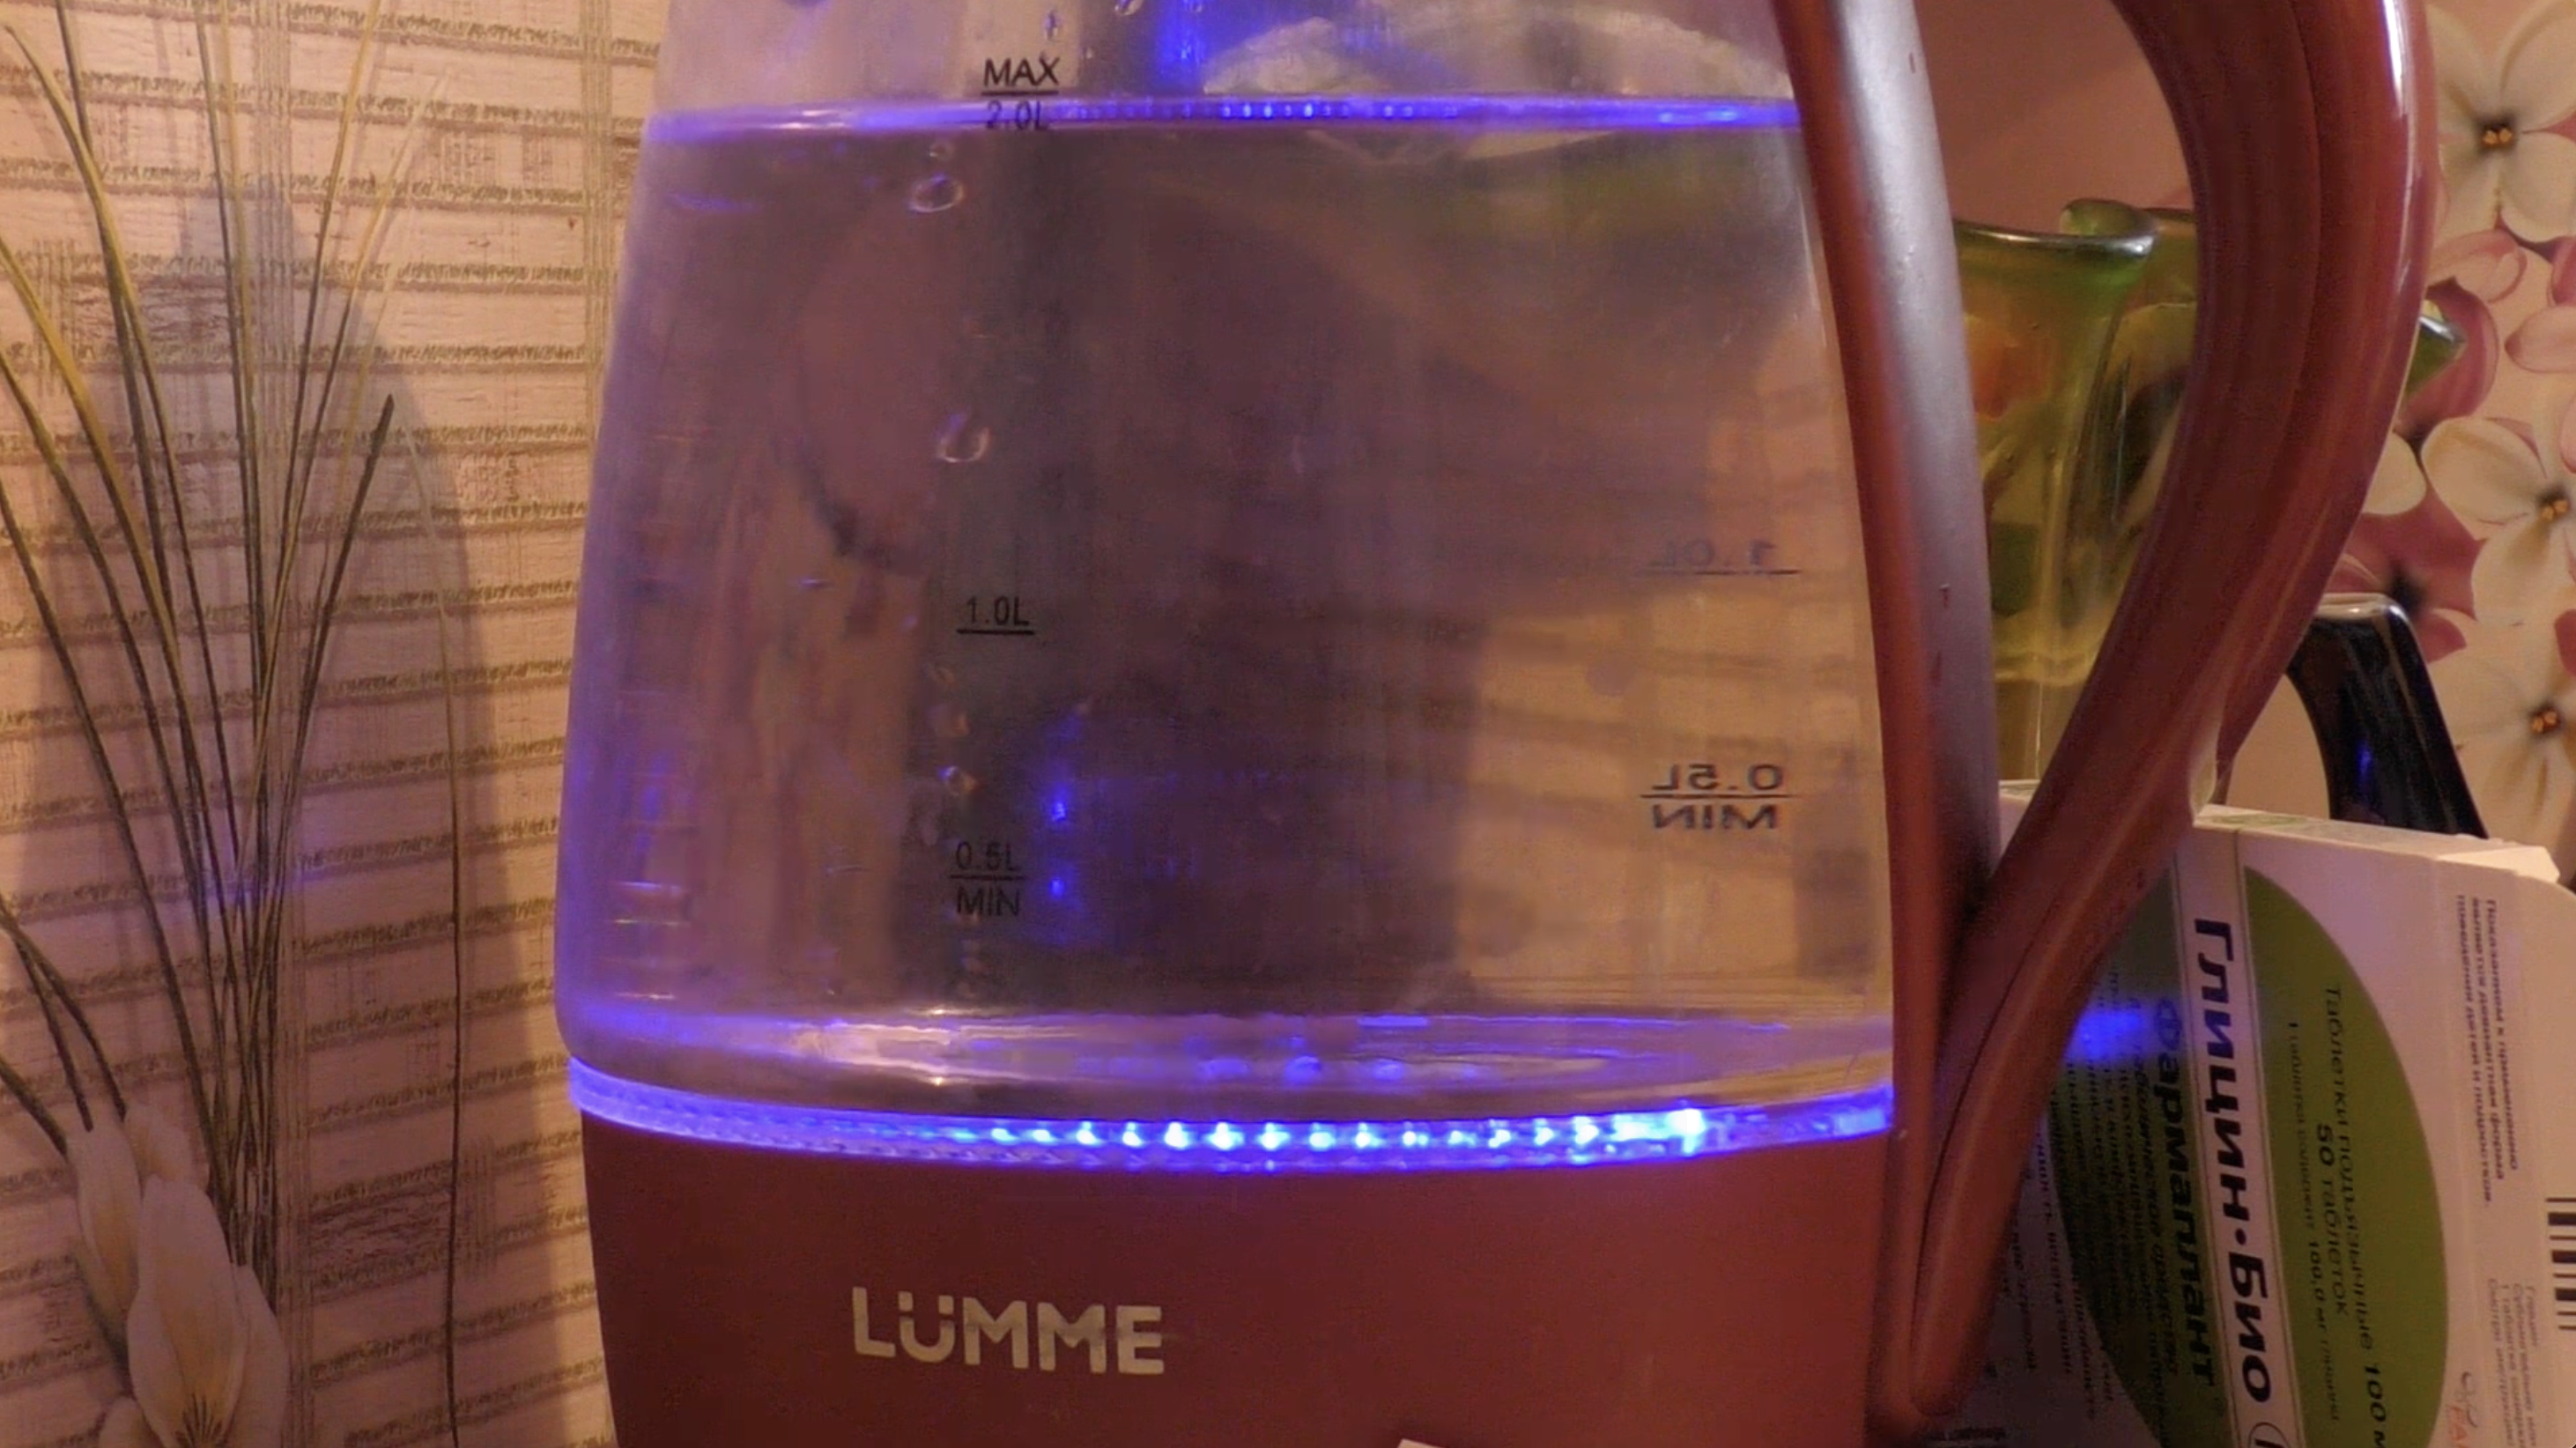
\includegraphics[width=0.8\textwidth]{images/image.png}
  \caption{Ошибка при вводе цепочки (cbaacbaab - верно, e - неверно)}
  \label{fig:image}
\end{figure}

\newpage
\section*{Заключение}
\addcontentsline{toc}{section}{Заключение}
В данной лабораторной работе была рассмотрена контекстно-свободная грамматика
(КС-грамматика) и реализован полный цикл построения LL(1)-анализатора
для неё.  
Были вычислены множества \textbf{FIRST} и \textbf{FOLLOW}.
На их основе сформирована таблица выбора (look-up table).
Отсутствие пересечений между множествами выбора альтернатив одного
нетерминала подтвердило, что грамматика принадлежит классу LL(1).

Каждой продукции назначено семантическое действие,
интерпретируемое как генерация точек на сетке и поиск пути между ними:
\texttt{generatePixel 0.3} для синих точек, \texttt{generatePixel 0.7} для зеленых
и \texttt{generatePixel 0.5} для оранжевых точек, с последующим поиском
кратчайшего пути между ними с использованием окрестности Мура.
\medskip
Для разбора был реализован детерминированный LL(1)-\emph{предиктивный анализатор}.

В ходе работы был реализован LL(1) парсер для заданной грамматики.

\begin{itemize}
\item \textbf{Плюсы}:
\begin{itemize}
    \item Сохранена грамматика LL(1).
    \item Разбирает входные цепочки и генерирует код для создания точек.
    \item Визуализирует точки на сетке и находит кратчайший путь между ними.
\end{itemize}


  \item \textbf{Минусы}
        \begin{itemize}
          \item Лексер тривиален: терминал \texttt{ab} должен
                вводиться как единая лексема, иначе разбор завершится
                ошибкой; для «настоящего» языка это потребует
                более гибкого токенизатора.
          \item Пришлось редактировать грамматику для корректного
                разбора. Не был реализован парсер для LL(3).
        \end{itemize}

  \item \textbf{Дополнения}
        \begin{enumerate}
          \item Усовершенствовать поиск минимальних путей алгоритмом A*.
          \item Добавить возможность вводить иные грамматики.
          \item Добавить возможность добавления "черных" точек в соответствии с грамматикой.
        \end{enumerate}
\end{itemize}

\newpage
\section*{Список литературы}
\addcontentsline{toc}{section}{Список литературы}
\begin{enumerate}
  \item Ю.Г. Карпов, Теория и технология программирования. Основы построения
  трансляторов. СПб.: БХВ-Петербург, 2005.
  \item А.В. Востров, "Математическая логика и теория автоматов". Распознавание КС-языков и трансляция. [Электронный ресурс], URL: https://tema.spbstu.ru/userfiles/files/courses/2018-compilers (дата обращения: 14.05.2025)
\end{enumerate}

\end{document}

